\chapter{提案手法の実装}
\section{点群モデルと取得}\label{sec:point-cloud}
	\subsection{点群について}
	手法1と手法2のどちらにおいても，容器の体積を計算するために容器モデルを計測することが必要である．
	また，今回の実装は容器の点群データを容器モデルとする．

	まず，点群データの取得設備について説明する．
	第3章で述べた通り，今回の実験ではロボットアームに取り付けたRealsenseD435というカメラで点群データを取得した．
	点群データはデプス画像とカメラの内部パラメータを用いて計算することで得られる．
	
	\subsection{容器点群モデルの取得する手法}\label{sec:get-model}
	容器の点群データから容器の体積を計算するためには容器の完全な点群が必要である．
	そして，多くの容器において単視点の撮影では完全な点群の取得がほぼ不可能である．
	そこで，今回の実験では完全な点群モデルを取得するため，容器の各方向から多視点の撮影を行う必要がある．
	
	具体的には，カメラのベース座標系の位置姿勢$^{b}T_{c} (p_\mathrm{center},\theta_\mathrm{view},\theta,r)$は以下の式を満たす：
	$$^{b}T_{c} (p_\mathrm{center},\theta_\mathrm{view},\theta,r)=\, ^{b}T_{vc}(p_\mathrm{center},\theta_\mathrm{view}) * ^{vc}T_{c}(\theta,r)$$
	ここで，$p_\mathrm{center},\theta,r,\theta_\mathrm{view}$はカメラの位置姿勢のパラメータ，$p_\mathrm{center}$はベース座標系の視点中心のxyz座標である．
	$\theta_\mathrm{view}$は視点方向の角度であり，視点座標系のz軸回りの回転角度である．
	$\theta$は視点の角度であり，カメラ座標系のy軸回りの角度である．
	$r$はカメラ座標系から視点座標系までの距離である．
	
	\begin{figure}[h]
		\centering
		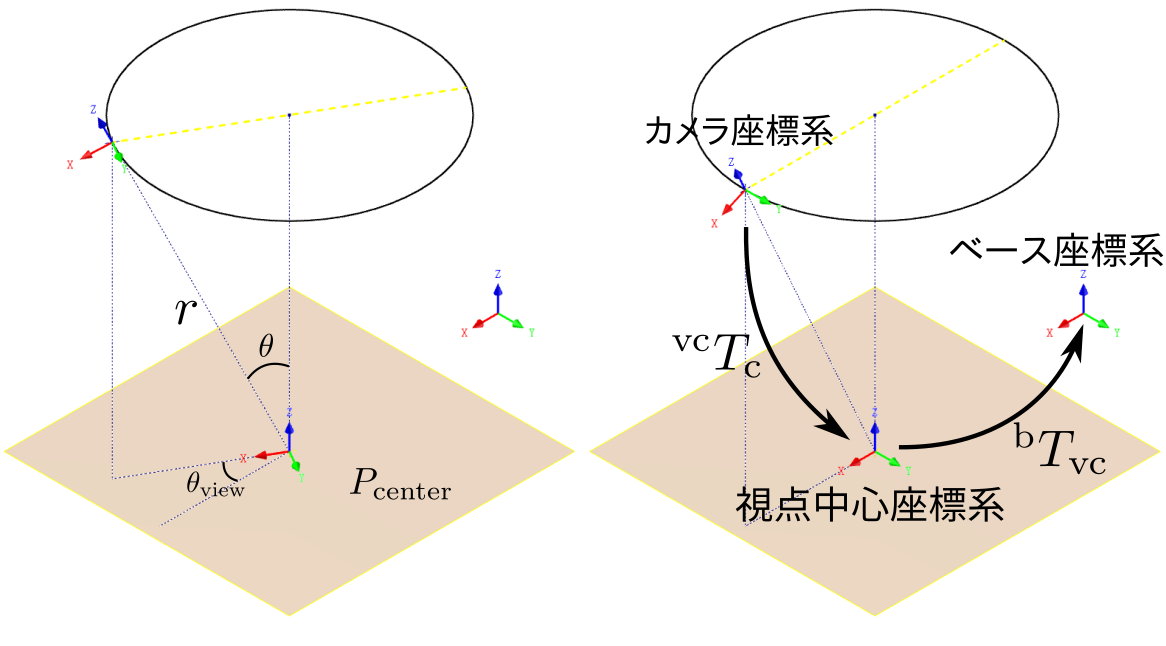
\includegraphics[width=0.8\linewidth]{fig/chp4/ViewPoint}
		\caption{視点の説明}
		\label{fig:ViewPoint}
	\end{figure}
	
	今回の実験において，$p_\mathrm{center}$は全て容器の中心で，$\theta_\mathrm{view}$は1周を12度間隔（合計30個）で選択される．\newline
	他のパラメータは：\newline
	手法1に対して，容器内側の点群が必要なため$\theta$は25度に設定し$r$は0.21[m]に設定した．\newline
	手法2に対して，容器外側の点群が必要なため$\theta$は65度に設定し$r$は0.17[m]に設定した．\newline
	$\theta$と$r$は，様々な撮影実験を行い，最適化された結果決まった値である．
	
	\subsection{多視点点群の合成}
	点群の合成は多視点点群を一つにする過程であり，各視点において不完全な容器の点群データを完全にすることである.
	
	合成する方法については，ICP(Iterative Closest Point)という，近い点群の間の位置回転関係を求める方法がしばしば用いられる．%TODO:添加ICP算法引用？
	しかし，ICPは初期位置に敏感な方法で，安定しないと考えたため今回は使用していない．
	
	今回の研究ではカメラがロボットの手先に取り付けてあるため，ロボットの手先の位置姿勢が分かれば，カメラの位置姿勢も知ることができる．
	そして，それぞれロボットの手先の位置姿勢で各視点の点群を世界座標系に変換すれば，全て合成することができる．
	具体的には，ある視点の左手のカメラで撮影した点群は以下の式で世界座標系に変換できることを利用する．
	\begin{equation}
		^wP =\:^wT_{lb}\:*\:^{lb}T_{lh}\:*\:^{lh}T_c\:*\:^cP
	\end{equation}
	ここで，$^wP$は世界座標系に変換した点群である．
	$^wT_{lb}$は左手ベース座標系から世界座標系に変換する変換行列である．
	$^{lb}T_{lh}$は左手の手先座標系から左手ベース座標系に変換する変換行列である．
	$^{lh}T_c$はカメラ座標系から左手の手先座標系に変換する変換行列で，
	$^cP$はRealsenseD435で取得したカメラ座標系の下での点群である．
	また，第2章の\ref{sec:robot}項の中央で述べた通り，世界座標系は左ロボットのベース座標系である．
	つまり，今回の実験では$^wT_{lb}$は単位行列である．
	次に，右手で撮影した点群について，第2章の\ref{sec:robot}項最後の段落で述べた両手の関係を参照し，右手ベース座標系から左手ベース座標系への変換行列$^{lb}T_{rb}$を求め，以下の式で合成する．
	\begin{equation}
	^wP =\:^wT_{lb}\:*\:^{lb}T_{rb}\:*\:^{rb}T_{rh}\:*\:^{rh}T_c\:*\:^cP
	\end{equation}
	
\section{体積の計算}
本節は\ref{sec:LiquidVolume}節の計算の実装方法について説明する．
	
	\subsection{点群のスライス方法と断面積の計算}\label{sec:slice}
	本項は\ref{sec:LiquidVolume}節の方法により，容器のモデルをスライスする方法について説明する．
	
	まず，スライスする高さを1[mm]とし，$z$軸に沿い，容器の$z_\mathrm{min}$から$z_\mathrm{max}$まで点群をスライスする．
	そして，1[mm]に満たないの部分の高さはそのままの高さにする．
	また，断面積を計算しやすくするために，各部分に含まれる全ての点を各部分底面のスライス平面に投影する．
	最後に，投影した各部分の点群を使用し，PCLにあるConvexHullというモジュールで，その部分の断面積を計算する．
		
\section{手法1実装：液面の高さに基づく注いだ体積の計算}
	\subsection{液面検出}\label{sec:pour-level-detect}
	本節は\ref{sec:Method1-liquidHeight}節の方法が必要とする液面高さの取得について説明する．
	
	まずは容器上から点群を撮影し，その点群から液面検出に関係ない点を除去する．
	液面検出は注いだ体積を計算するプログラムに必要となるため，また，注いだ体積の計算は注ぎ作業をしている間リアルタイムに動作しているため，液面検出についてもリアルタイム性が必要と考えられる．
	そこで，容器の世界座標系下で，容器モデルを取得した時に計算されたAABB(Axis Align Bounding Box)バウンディングボックスを使用する．
	注ぎ先の容器の上から撮影した点群に対してPCLのPassThroughフィルターを使うことで，バウンディングボックス以外の点を全て除去する．
	
	そして注ぎ先の容器上部に残された点群をPCLの平面抽出モジュールを使用し，点の数が最大の平面を液面とし，それを抜き出し，それらの点のz座標の平均を液面の高さとする．
	
	\subsection{変換テーブル}\label{sec:Method1-Table}
	プログラムを高速化するため，液面の高さから注いだ体積への変換テーブルを作成した．
	\ref{sec:LiquidVolume}節で提案した手法は各断面の面積を計算する必要があるため，リアルタイムで計算するのは難しいと考えられる．
	そこで，液面の高さからその高さに対応する体積への変換テーブルを容器のモデルを分析する際に作成しておく．
	注ぐ際には，液面の高さを計測すれば，テーブルを参照することで注がれた液体の体積が求められる．
	
	また，注ぐ際には，液面の高さは時間とともに連続して変化していく．
	しかし，変換テーブルは連続ではない．
	そこで，連続な液面の高さ$h$に対して，最終的な体積の結果は線形補間を使い，以下の式で求める．%TODO:液面高跟体积变换表的线性插值公式。
	\begin{equation}
	V_\mathrm{output} = T(\lfloor h \rfloor) + \Big(T(\lceil h \rceil ) - T(\lfloor h \rfloor)\Big)\cdot\Big( \frac{h - \lfloor h \rfloor}{\lceil h \rceil  - \lfloor h \rfloor}\Big) \label{exp:Method1-Table}
	\end{equation}

	
\section{手法2実装：注いだ体積と注ぐ容器の傾き角度の関係による注いだ体積の計算}\label{sec:Method2Real}
	\subsection{初期液体の体積の計算}
	初期液体の体積を計算する方法は\ref{sec:Method1-liquidHeight}節の方法である．
	その方法を使用するには初期液面の高さと注ぐ容器のモデルが必要である．
	そして，液面の高さは\ref{sec:pour-level-detect}節の手順で検出する．
	次に，容器の初期状態がすでに液体が入っている状態であるため，容器モデルを得るために容器内部の点群を取得することは困難である．
	そこで，手法2の一部実験(\ref{sec:Method2-expAll}節)では容器外側の点群を容器のモデルとして使用する．
	
	\subsection{注ぎ縁の検出}
	注ぎ縁の検出の流れは：
	まず，あるモデルの姿勢を選び，その姿勢の変換行列で注ぐ容器のモデルを変換する．
	次に，点群モデルをz軸に沿ってスライスし，断面の不連続な部分の端点を検出する．
	さらに，検出した点をその姿勢の逆変換行列で逆変換する．
	以上の手順を全ての姿勢で完了するまで繰り返す．
	
	\subsubsection{断面の不連続な部分の端点の検出}
	本節は容器モデルの断面において，断面形状の不連続な部分の端点を検出する方法について説明する．
	断面の取得は\ref{sec:slice}節の方法と同じである．
	
	不連続な部分の端点は断面形状の方向(図\ref{fig:pour-edge-detect-1}の線の方向)に沿い，隣接する点の距離がしきい値より大きい2つの点である(図\ref{fig:pour-edge-detect-1}の丸がついた点)．
	\begin{figure}[hp]
		\centering
		
\includegraphics[width=0.5\linewidth]{fig/chp4/PourEdgeDetect}
		\caption{不連続な部分の端点の説明}
		\label{fig:pour-edge-detect-1}
	\end{figure}
	
	しかし，点群の順番はランダムで，断面の形状に沿うことができない．
	そこで，PCLのConvexHullというモジュールを使用し，断面点群のConvexHullを計算する．
	\begin{figure}[hp]
		\centering
		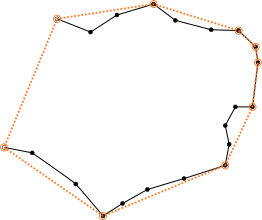
\includegraphics[width=0.5\linewidth]{fig/chp4/PourEdgeConvexHull}
		\caption{ConvexHullの結果}
		\label{fig:pour-edge-1}
	\end{figure}
	図\ref{fig:pour-edge-1}で，オレンジの丸の点とオレンジの破線はConvexHullの結果であり，オレンジの丸の点の順番も破線の方向に修正した．
	
	次に，ConvexHullの結果から，隣接する2点を取り出し，その間で不連続な部分の端点を検出する．
	検出する方法は：
	\begin{figure}[hp]
		\centering
		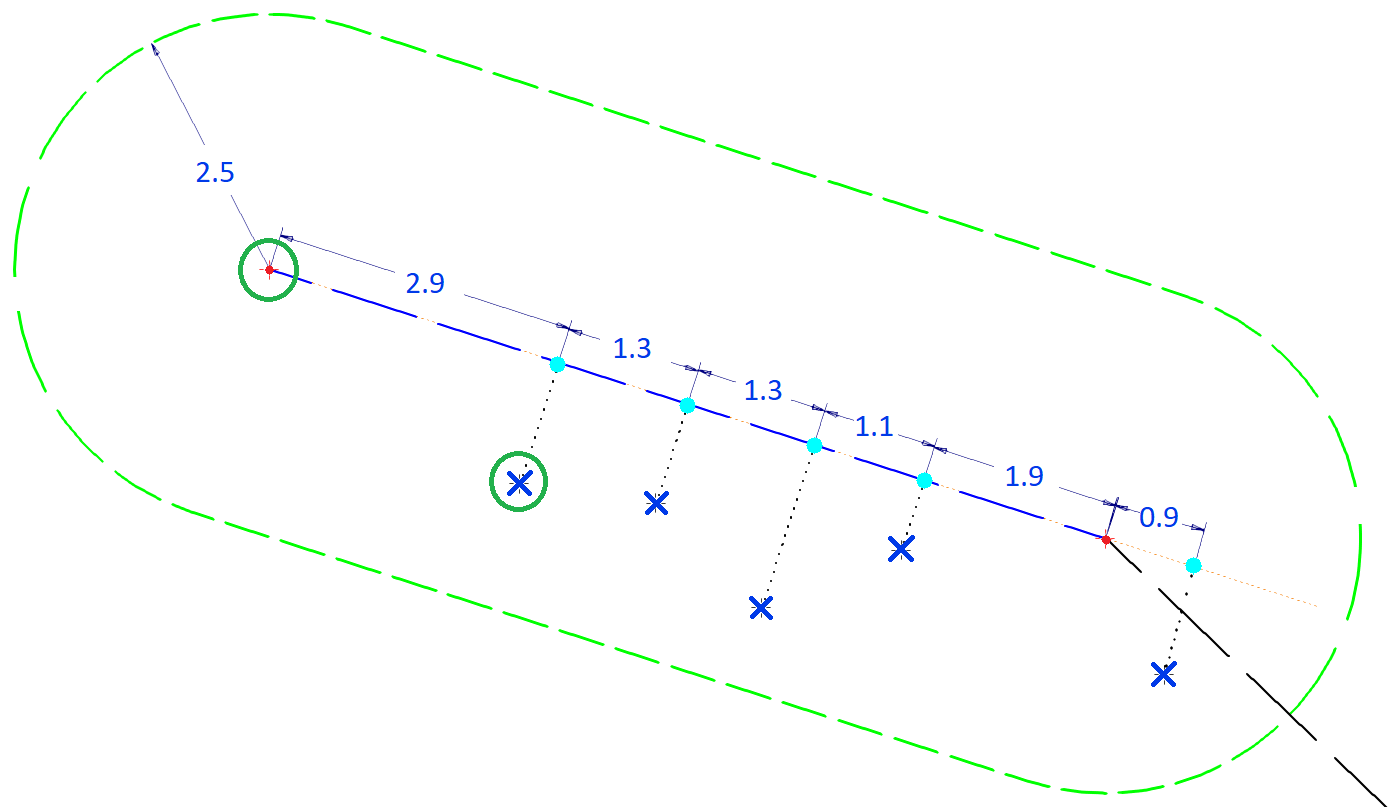
\includegraphics[width=0.8\linewidth]{fig/chp4/pour-edge-2}
		\caption{不連続な部分の端点の計算}
		\label{fig:pour-edge-2}
	\end{figure}

	\begin{enumerate}
		\item 隣接する2点(赤色の点)で引かれる直線(図\ref{fig:pour-edge-2}の青い破線)の，半径2.5[mm]の範囲内(図\ref{fig:pour-edge-2}の緑色の破線)の点をすべて取り出す．
		\item 取り出した点を手順1の直線(図\ref{fig:pour-edge-2}の青い破線)に投影する(図\ref{fig:pour-edge-2}の青い点)．
		\item 投影した各点の間の距離を計算する(図\ref{fig:pour-edge-2}の寸法)．
		\item 投影した各点が隣接する2点間にある点かを判断する．投影した点から隣接する2点の距離を足し算した結果が隣接する2点の間の距離より大きければ，この点は隣接する2点の間の点ではないと判断し，計算手順から除く．
		\item 投影した点の間の距離がしきい値より大きければ，その2点を不連続な部分の端点とする(しきい値は2.5[mm]で，図\ref{fig:pour-edge-2}の深い緑の円で囲まれた範囲)．
	\end{enumerate}

	\subsubsection{注ぎ縁のノイズ処理}
	上の方法で計算した注ぎ縁はノイズがある(図\ref{fig:pour-edge-noise})．
	\begin{figure}[h]
		\centering
		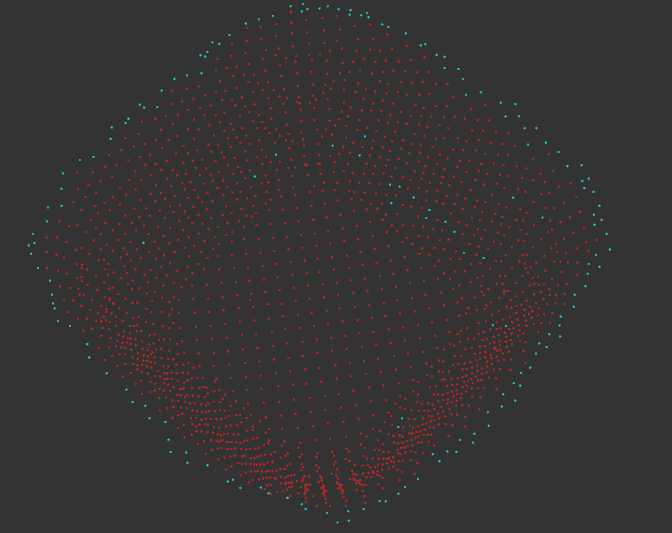
\includegraphics[width=0.6\linewidth]{fig/chp4/pour-edge-noise}
		\caption{注ぎ縁のノイズ(容器3の上から撮影)}
		\label{fig:pour-edge-noise}
	\end{figure}
	
	処理しない場合，次の注ぐポイントの検出に影響がある．
	そこで，PCLのEuclideanClusterExtractionというモジュールを使用し，注ぎ縁の点群をクラスタリングする．
	そして，クラスタの中で，平均高さと点数が一番高いクラスタを注ぎ縁とする．
	
	\subsection{注ぐポイントの検出}
	検出した注ぎ縁を使用し，注ぐ方向(本論文はx軸回り)に回転しながら，各傾き角度の注ぎ縁の最低点を取り出す．
	そして，PCLのEuclideanClusterExtractionというモジュールを使用し，取り出した点をクラスタリングする．
	最後に，クラスタの中で，平均高さが一番低いクラスタの中心を注ぐポイントとする．
	
	\subsection{注ぐ方向に対する注いだ体積と注ぐ容器の傾き角度の関係の計算}\label{sec:Method2-TableCal}
		\subsubsection{傾き角度から注いだ体積への変換テーブルのノイズ処理と連続化}
		\ref{sec:LiquidVolume}や
		\ref{sec:pour-point-detect}		節に書いた方法で，傾き角度から注いだ体積への変換テーブルが計算できる．
		
		しかし，点群モデルのノイズの影響で，傾き角度の増加とともに，計算上の注いだ体積が減少する場合がある．
		実際の注ぎ作業においては，傾き角度が増加している状態で注いだ体積が減少することはない．
		したがって，ノイズを処理しないと，誤差の原因となってしまう．
		
		そこで，傾き角度から注いだ体積への変換テーブルにおいて，線形補間を使用する．注いだ体積の減少が始まると，減少が終わるまでのデータを入れ替える．
		\begin{figure}[h]
			\centering
			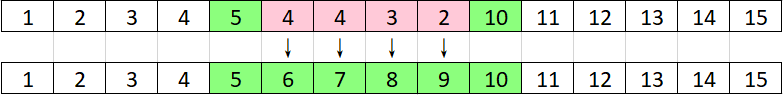
\includegraphics[width=0.8\linewidth]{fig/chp4/linerInterp}
			\caption{線形補間}
			\label{fig:pour-angle-noise-linerInterp}
		\end{figure}
		
		傾き角度から注いだ体積への変換テーブルの連続化について，	\ref{sec:Method1-Table}節の式\ref{exp:Method1-Table}で変換テーブルを連続化する．
		
		\subsubsection{注いだ体積から傾き角度への変換テーブルの計算}
		今まで，傾き角度から注いだ体積への変換テーブルの計算と修正をした．
		しかし実際に注ぐ時には，注いだ体積から傾き角度への変換テーブルが必要である．
		
		そこで，注いだ体積と傾き角度の関係が必ず増加する関係という条件を利用し，バイナリサーチを使用し，注いだ体積に対応する傾き角度を探す．
	
% \section{容器の掴み方}
% 掴み方は\ref{sec:endeffector}節二種類のエンドエフェクタに応じて，二種類がある．
% その一は大きな容器に対して，注ぎ縁を掴むことである．
% その二は小さな容器に対して，外側から掴むことである．

% 	\subsection{その一：注ぎ縁を掴む}
% 	この方法は回転なし，ロボットの視点から注ぎ縁一番右の位置を掴む方法である．
	
% 	\ref{sec:pour-edge-detect}節で提案した方法で注ぎ縁を検出した後，y軸方向に最小(ロボットの視点から一番右の位置)の点を取り出す．
% 	そして，その点の座標をロボット手先の目標位置とし，手先の回転オイラー角度$\alpha, \beta, \gamma$は全部ゼロとする．
	
% 	\subsection{その二：外側から掴む}
% 	PCL主成分分析のモジュールを使い，掴む容器の中心を分析し，ロボットのツール座標系を容器の横から中心と合成するように動き，グリッパが閉めれば，容器を掴むことができる．
	
% 	なぜ横から掴むのは，上から掴むなら，図\ref{fig:hardtopour}のように，ロボットの手先とテーブルや容器がぶつかる可能性があるため，注ぎ作業が非常に困難になる。
% 	\begin{figure}[h]%TODO:竖直抓取困难图
% 		\centering
% 		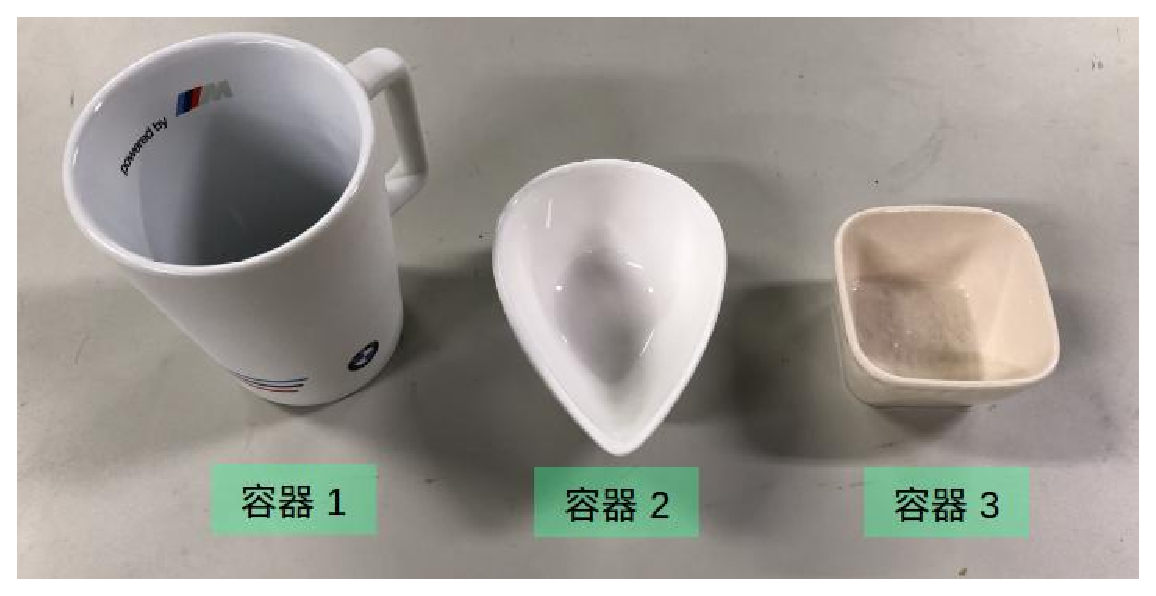
\includegraphics[width=0.4\linewidth]{fig/chp5/Cups-v2}
% 		\caption{注ぎ作業が非常に困難}
% 		\label{fig:hardtopour}
% 	\end{figure}
% 	また，注ぎ作用において，注ぎ先容器が掴まれながら注がれる場合より，注ぐ容器を掴んだ場合のほうが多い．
	
	
	
	